\section{Considerações Iniciais}\label{sec:consideracoes_iniciais}
Geralmente refatorações são aplicadas para melhorar a qualidade do software (por exemplo, a extensibilidade, a modularidade, a capacidade de reutilização, a complexidade, manutenção, etc). 
A maioria das pesquisas apontam que usualmente refatorações são aplicadas em nível de código-fonte~\cite{Fowler1999, Demeyer1, Demeyer2, OPDYKE_1992}. Tais pesquisas não estão preocupadas em como promover o reuso, compartilhamento de refatorações e também não estão interessadas em criar refatorações para outros tipos de artefatos, tais como os artefatos providos pela ADM, por exemplo, o metamodelo KDM. 
%
Como já destacado, na literatura é possível identificar um conjunto de refatorações já validadas e que são usualmente aplicadas em código-fonte, por exemplo, \textit{Extract Class}, \textit{Move Method}, \textit{Move Attribute}, etc. Essas são apenas alguns exemplos de refatorações úteis que não são facilmente reutilizadas na prática durante a condução de modernização de um determinado sistema. Essa limitação pode ser atribuída devido a ausência de um meio padronizado de disponibilizar refatorações. 
Uma abordagem promissora é lidar com a refatoração de forma independente da linguagem – aumentando assim as possibilidades de reutilização de refatorações.

Como ressaltado no Capítulo~\ref{chapter:fundamentacao_teorica} a ADM fornece um conjunto de metamodelos para auxiliar o engenheiro de software a conduzir MDE. 
Porém, até esse momento a ADM não possui instruções ou até mesmo um metamodelo para auxiliar o engenheiro de modernização a promover o reuso de refatorações juntamente com os seus metamodelos padronizados (por exemplo, KDM) durante o processo de modernização. 
Essa limitação faz com que o engenheiro de modernização crie suas próprias soluções/refatorações, resultando em um possível atraso no processo de modernização. 
No Capítulo~\ref{chapter:catalogo_refactoring_KDM} algumas refatorações bem conhecidas e propostas por~\citeonline{Fowler1999} são adaptadas para serem aplicadas em instâncias do metamodelo KDM. Contudo, em seu estado atual as refatorações adaptadas não podem serem facilmente reutilizadas e compartilhadas entre os modernizadores. 
Com o intuito de suprir tal limitação neste capítulo é apresentado um metamodelo para auxiliar o engenheiro de modernização a promover o reuso de refatorações no contexto do metamodelo KDM. Com a utilização desse metamodelo, informações (metadados) sobre refatorações podem ser reutilizadas de forma independente de linguagem e plataforma. Além do metamodelo criado esse capítulo também apresenta a metodologia empregada para a sua criação. Acredita-se que os passos utilizados na metodologia podem ser replicados para auxiliar outros engenheiros de modernização durante a criação de novos metamodelos no contexto da ADM.

O metamodelo aqui proposto tem as seguintes características: (\textit{i}) permite a interoperabilidade de refatorações para um amplo domínio e (\textit{ii}) auxilia o engenheiro de modernização a definir refatorações representativas em forma de metadados. Nota-se que o metamodelo aqui proposto segue a mesma proposta de outros metamodelos definidos na ADM e está totalmente integrado com o metamodelo KDM. Em outras palavras, uma instância do metamodelo de refatoração contém metadados que representam uma refatoração escrita para ser executada em uma instância do metamodelo KDM. A escolha do metamodelo KDM se deu pois o mesmo é um metamodelo padronizado pela OMG, além de ser um metamodelo PIM, o que significa que quaisquer refatorações aplicadas em uma instância do KDM, podem ser consideradas independentes de linguagem e de plataforma e então ser transformado para em um PSM (ver Capítulo~\ref{chapter:fundamentacao_teorica}). Utilizar refatorações como um metamodelo (de forma independente de linguagem) pode abrir opções para promover o reuso de refatorações. Por exemplo, dado uma instância do metamodelo de refatoração, o engenheiro de modernização poderia utilizar os metadados contidos nessa instância e aplicar a refatoração em qualquer sistema representado pelo KDM. Além disso, o engenheiro de modernização poderia instanciar o metamodelo de refatoração, criar um catálogo de refatorações e disponibilizar para que outros possam reutilizar tais refatorações. Tornando assim possível compartilhar e reutilizar refatorações no contexto da ADM.

%Com o intuito de apresentar o metamodelo de uma maneira mais prática, neste capítulo a construção do mesmo é realizado com o uso do EMF~\cite{EMF}. Porém, ressalta-se que o metamodelo pode ser criado com o uso de outras tecnologias.

As demais seções deste capítulo estão organizadas da seguinte forma: na Seção~\ref{sec:motiva_o_para_a_cria_o_de_um_meta_modelo_de_refatora_o} são destacadas as principais motivações para criar um metamodelo para prover o reúso de refatorações; na Seção~\ref{sec:meta_modelo_de_refatora_es_estruturadas_srm_do_ingl_s_structured refactoring meta-model_} o Metamodelo de Refatorações Estruturadas é apresentado, destacando os principais passos para a engenharia do metamodelo SRM; na Seção~\ref{sec:implementacao_do_SRM}  é destacado como o metamodelo SRM foi implementado, além disso, é também apresentado a gramática de uma DSL criada com o propósito de auxiliar a instanciação do metamodelo SRM; na Seção~\ref{sec:trabalhos_relacionais_SRM} alguns trabalhos relacionados são apresentados; e na Seção~\ref{sec:consideracoes_finais_SRM} são feitas as considerações finais a respeito do metamodelo de refatoração proposto neste capítulo.

\section{Motivação para a criação de um metamodelo de refatoração} % (fold)
\label{sec:motiva_o_para_a_cria_o_de_um_meta_modelo_de_refatora_o}

Durante o mapeamento sistemático conduzido (ver Capítulo~\ref{chapter:mapeamento_sistematico})~\cite{durelli_systematic_mapping} pôde-se observar na literatura a carência de estudos que definem soluções para especificar e promover o reuso de refatorações no contexto da ADM e do metamodelo KDM. Sem a adequada representação de refatorações para o KDM, a especificação e realização de uma refatoração pode se tornar uma atividade propensa a erros e difícil de reutilizar.

Neste contexto, suponha o seguinte cenário, um engenheiro de modernização define uma determinada refatoração e a compartilha por meio de um repositório. Dessa forma, outros engenheiros podem então navegador nesse repositório e identificar, não apenas essa, mas um conjunto de refatorações. O engenheiro então escolhe uma determinada refatoração no repositório, faz o \textit{download} e a reutiliza em seu sistema representado em nível de uma instância do metamodelo KDM. 

Uma das soluções para a concretização desse cenário seria a criação de um metamodelo para persistir metadados referentes à refatorações. Esse metamodelo deve possuir metaclasses e meta-relacionamentos que permitam representar e especificar metadados de refatorações, por exemplo, o nome da refatoração, sua motivação, os passos para sua realização, e até mesmo o mecanismo e sua pré- e pós-condições. Devido a carência de um metamodelo que possui tais particularidades, esse capítulo tem como principal objetivo definir e apresentar um metamodelo que permita a representação de metadados relacionadas com refatorações, porém, ainda respeite e siga as características dos metamodelos definidos na abordagem ADM, por exemplo, o metamodelo aqui definido precisa ser independente de linguagem e plataforma.

Essa última características é de suma importância. Assim, o metamodelo aqui apresentado utiliza as metaclasses do metamodelo KDM. Uma instância do metamodelo de refatoração, deve possuir instâncias de metaclasses específicas para definir metadados sobre refatorações (autor, nome, motivação, descrição, etc) e também instâncias de metaclasses do KDM que representam os elementos estruturais (\texttt{ClassUnit}, \texttt{StorableUnit}, \texttt{MethodUnit}, etc) onde a refatoração/transformação será aplicada. Dessa forma, o metamodelo de refatoração faz com que a operação/mecanismo de uma refatoração torne-se independente de plataforma e linguagem de programação. Assim, o metamodelo pode ser facilmente utilizado e aplicado em ferramentas existentes que utilizam como base o KDM aumentando a interoperabilidade de futuras ferramentas que utilizem esse metamodelo de refatoração. Levando em consideração as motivações destacadas, na Seção~\ref{sec:meta_modelo_de_refatora_es_estruturadas_srm_do_ingl_s_structured refactoring meta-model_} é apresentado o metamodelo de refatorações estruturadas (do inglês - Structured Refactoring Metamodel – SRM).  


%Além disso, uma característica de suma importância é que esse metamodelo de refatoração seja baseado nas metaclasses do KDM. Em outras palavras, uma instancia desse metamodelo, deve conter referencias a metaclasses do KDM, tornando assim, a operação/mecanismo de um refatoração independente de plataforma e linguagem. 

\section{Metamodelo de Refatorações Estruturadas} % (fold)
\label{sec:meta_modelo_de_refatora_es_estruturadas_srm_do_ingl_s_structured refactoring meta-model_}

Como pôde ser observado na seção anterior, são várias as motivações para definir um metamodelo para especificar refatorações. Neste sentido, nesta seção é apresentado um metamodelo denominado Metamodelo de Refatorações Estruturadas (do inglês - \sigla{SRM}{\textit{Structured Refactoring Metamodel}}).

Refatorações são ubíquas durante a manutenção, produção e análise de software. Inúmeras comunidades têm surgido na literatura para criar e definir vários tipos de refatorações, incluindo refatorações de baixa granularidade~\cite{Fowler1999, Demeyer1, Demeyer2}, refatorações arquiteturais, refatorações para o paradigma orientado a aspecto, etc. Neste contexto, existe a necessidade de definir uma forma de promover o compartilhamento dessas refatorações. Assim, nessa seção é apresentado um metamodelo para auxiliar tais comunidades. Esse metamodelo representa uma fundamentação para o compartilhamento de informações (metadados) relacionadas à refatorações, assim, detalhes com informações precisas sobre refatorações podem ser armazenadas e/ou compartilhadas para que outros engenheiros possam reutilizar em seus projetos que utilizem o metamodelo KDM.

Por exemplo, uma comunidade que cria refatorações de baixa granularidade usualmente esta preocupada em definir e especificar refatorações desse tipo. Por outro lado, uma comunidade que especifica refatorações arquiteturais esta interessada apenas em refatoração arquiteturais. Porém, nota-se que ambas comunidades têm em comum a necessidade de especificar como organizar e definir as refatorações. Além disso, tais comunidades devem se preocupar em definir a motivação para a condução da refatoração, especificar o mecanismo da refatoração e descrever tais refatorações de maneira formal e adequada para a sua comunidade. Embora o contexto dessas comunidades seja diferentes ambas necessitam de uma forma padronizada para definir e especificar as refatorações. 


O SRM define um padrão comum para a especificação e descrição de refatorações. Além disso, esse metamodelo tem como princípio ser independente de linguagem de programação com o objetivo de fornecer uma plataforma comum pelo qual arquiteto, pesquisador e modernizador possam expressar refatorações sem se preocuparem com a plataforma ou linguagem de programação. O SRM possui três principais objetivos: (\textit{i}) prover uma forma de compartilhar informações sobre refatorações; (\textit{ii}) promover o reuso de refatorações de forma independente de plataforma e linguagem; e (\textit{iii}) ser uma proposta inicial ao \textit{Call for Proposals} do ADM \textit{Refatoring} do OMG. O primeiro objetivo é apoiada por um conjunto de metaclasses que definem meta-atributos específicos para representar informações (metadados) de uma refatoração, auxiliando assim o compartilhamento das refatorações de forma intuitiva para os modernizadores. Similarmente, o segundo objetivo também é alcançado por metaclasses que possuem meta-atributos que representam os mecanismos das refatorações, bem como suas pré- e pós-condições. O terceiro objetivo é apoiado por todo o metamodelo SRM.
 
Na Figura~\ref{fig:refactoring_metamodel} o SRM é esquematicamente apresentado. O centro da figura representa a abordagem ADM. Pode-se entender que o SRM está inserido no contexto da ADM da mesma forma que seus outros metamodelos. A esfera externa é dividida em quatro facetas, cada faceta possui o nome de um metamodelo – por sua vez, cada faceta é acoplada por um retângulo contendo o nome de um metamodelo e um conjunto de metaclasses. Como pôde ser observado nessa figura o SRM está inserido no contexto da ADM para preencher a definição de um metamodelo de refatorações. 

\begin{figure}[h]
	\centering
	% Requires \usepackage{graphicx}
	\caption{Integração do SRM com outros metamodelos da ADM.}
	\label{fig:refactoring_metamodel}
	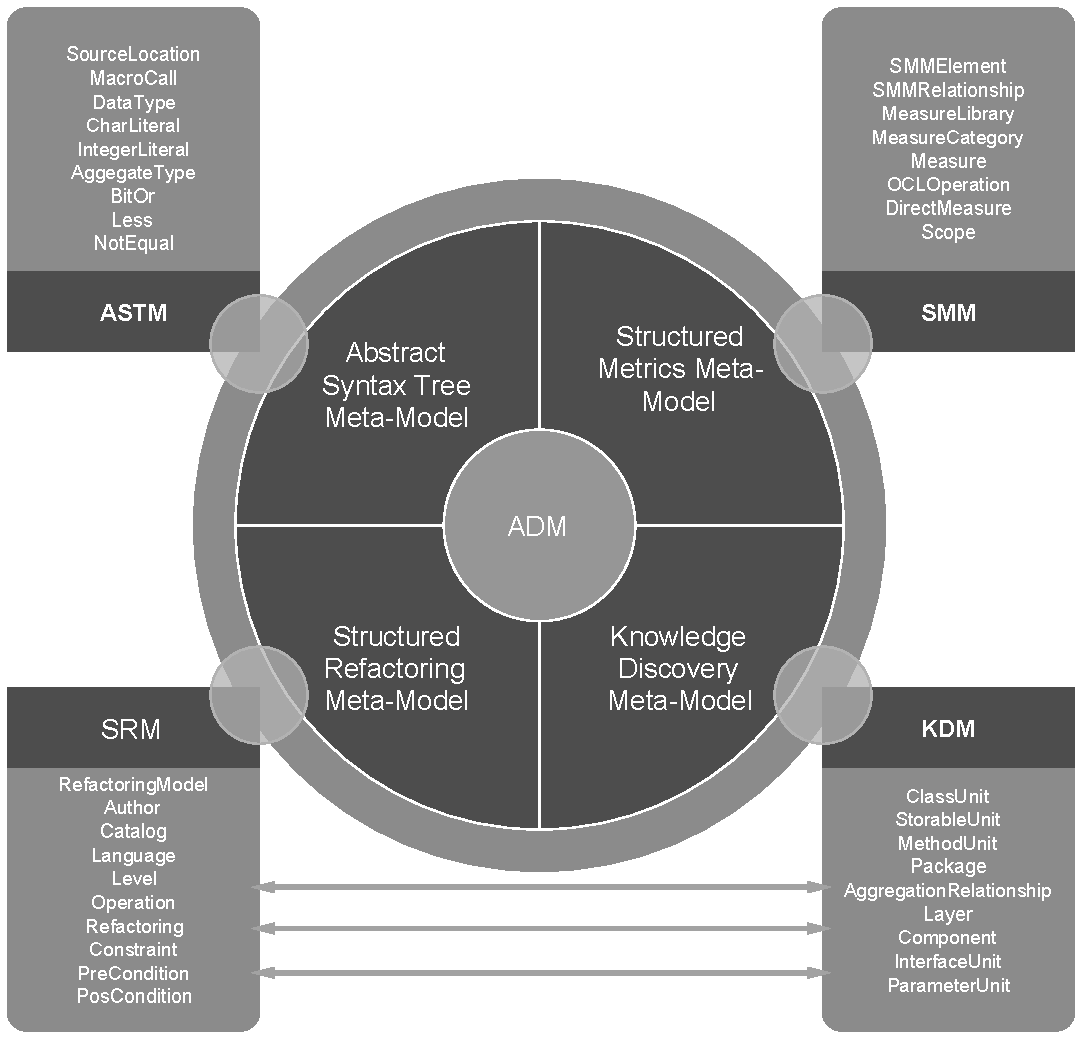
\includegraphics[scale=0.6]{images/SRM2Formatted}
	\fautor
\end{figure}

Um dos objetivos do SRM é seguir as padronizações propostas pela ADM. Porém, deve-se ressaltar que o SRM é utilizado para especificar a representação de refatorações sem se preocupar com a representação das partes estruturais de uma refatoração, ou seja, os elementos que serão refatorados (classes, métodos, atributos, etc.). Assim, o SRM assume que tais elementos (classes, métodos, atributos, etc.) devem ser representados utilizando outro metamodelo proposto pela ADM, neste contexto o KDM. Como visualizado na Figura~\ref{fig:refactoring_metamodel}, o SRM interage com o metamodelo KDM para utilizar instâncias de metaclasses do KDM para representar os elementos que serão refatorados. Consistente com outros metamodelos definidos pela OMG, o SRM é definido utilizando a padronização de modelagem MOF e a \textit{framework} EMF. Um dos benefícios de utilizar MOF é que o mesmo permite que o metamodelo seja serializado e deserializado sem perder nenhum tipo de informação, ou seja, metamodelos instanciados são representados utilizando uma representação textual padronizada, XMI. Além disso, o SRM é compatível com repositórios MOF para armazenamento e recuperação de várias ferramentas, aumentando assim a interoperabilidade de futuras ferramentas que utilizem esse metamodelo.

\begin{figure}[h]
	\centering
	% Requires \usepackage{graphicx}
		\caption{Visão completa do metamodelo SRM.}
	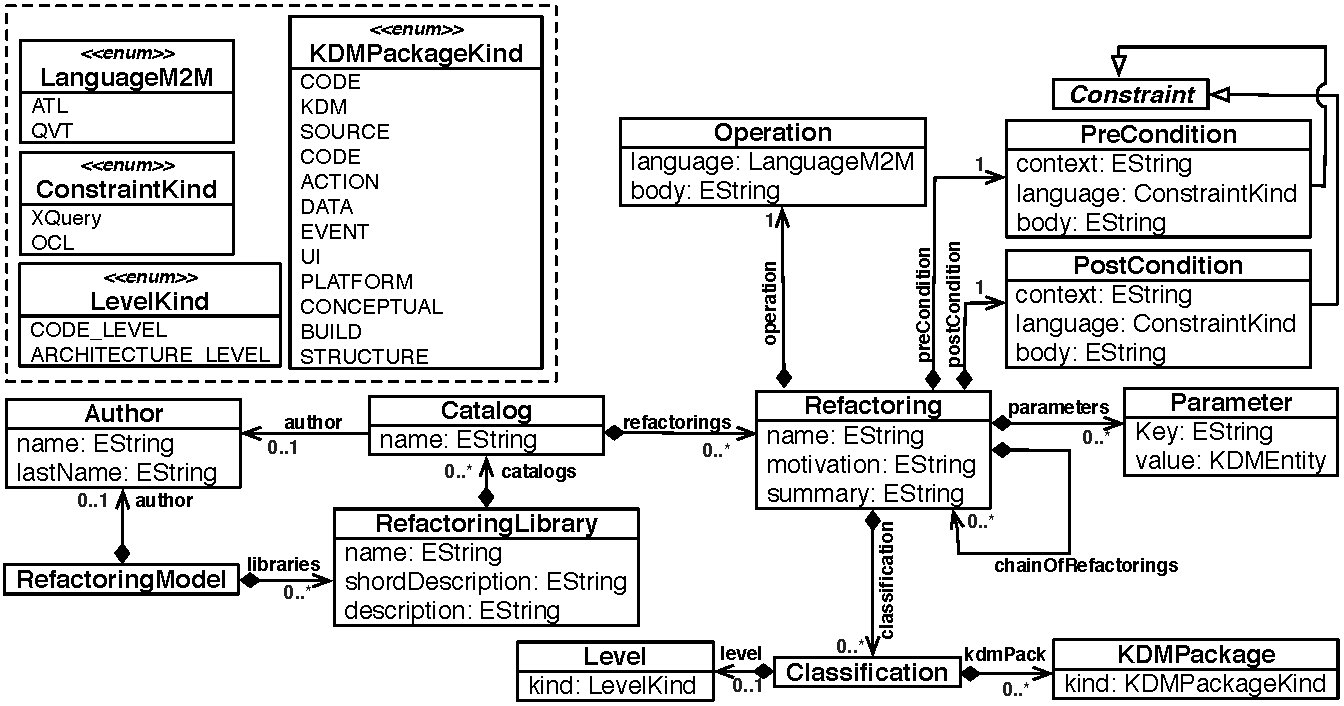
\includegraphics[scale=0.65]{images/newMetamodelSRM}
	\label{fig:meta_modelo_SRM}
	\fautor
\end{figure}

O metamodelo SRM é apresentado na Figura~\ref{fig:meta_modelo_SRM}. Esse metamodelo contém três pacotes, 13 metaclasses e quatro enumerações. Na Figura~\ref{fig:fases_para_a_construcao_e_uso_do_SRM} é apresentada uma macro-visão da engenharia do metamodelo SRM utilizando a notação SADT. Como observado um conjunto de elementos foram utilizados como base para o desenvolvimento do SRM: elementos estruturais, linguagens de transformações, linguagens de restrições e catálogos de refatorações. %A seguir, na Subseção~\ref{Engenharia_do_Meta_modelo_SRM} esses elementos são apresentados e comentados como foram utilizados para desenvolver o metamodelo SRM.

\begin{figure}[h]
	\centering
	% Requires \usepackage{graphicx}
	\caption{Macrovisão para a construção do SRM.}
	\label{fig:fases_para_a_construcao_e_uso_do_SRM}
	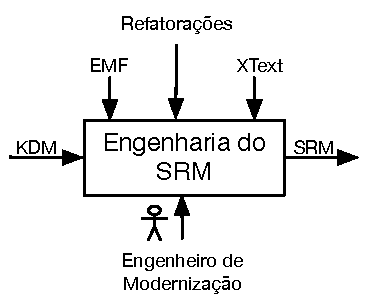
\includegraphics[scale=0.9]{images/engenhariaDoSRM}
	\fautor
\end{figure}

%\section{Engenharia do SRM}\label{Engenharia_do_Meta_modelo_SRM}

Refatorações, suas características e terminologia foram analisadas para que o SRM fosse desenvolvido. Antes de iniciar a criação do metamodelo SRM (ou de qualquer outro metamodelo) é necessário definir os elementos que deverão ser representados e as relações entre eles. Nesse sentido, três principais passos que compõem a engenharia do SRM são mostradas na Figura~\ref{fig:etapas_da_fase_de_e_do_SRM}: (\textit{i})  Identificar vocabulário/termos/conceitos, (\textit{ii}) Projetar e criar o SRM e (\textit{iii}) Implementar o SRM. Cada passo da metodologia utilizada para criar o SRM é apresentado com mais detalhes a seguir.

\begin{figure}[h]
	\centering
	% Requires \usepackage{graphicx}
	\caption{Metodologia empregada na criação do metamodelo SRM.}
	\label{fig:etapas_da_fase_de_e_do_SRM}
	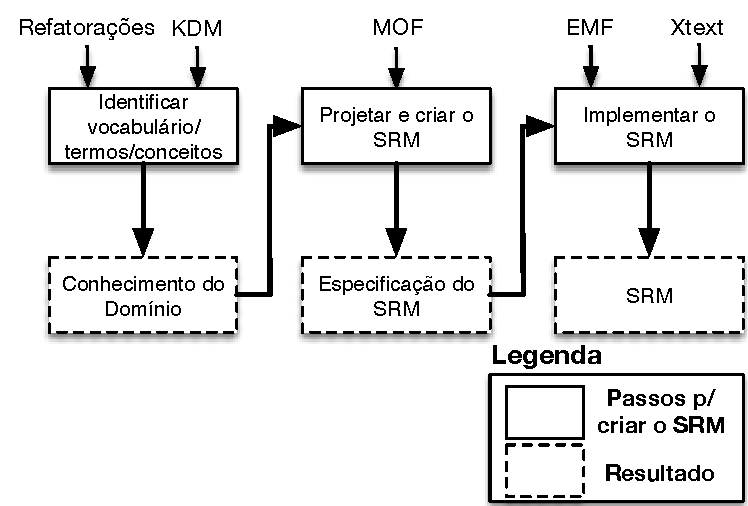
\includegraphics[scale=0.65]{images/metodologiaParaCriarOSRM}
	\fautor
\end{figure}



\subsection{Identificar vocabulário/termos/conceitos}

Neste passo é realizada a identificação do vocabulário, termos e conceitos comuns que são utilizadas dentro da comunidade de refatoração. Durante a criação de metamodelos é de suma importância entender o domínio que o metamodelo representa. metamodelos definem abstrações (termos), notações e relacionamentos para representar um determinado domínio. Assim, neste passo tanto os vocabulários, termos e conceitos definidos por~\citeonline{OPDYKE_1992} e \citeonline{Fowler1999} foram analisados para a identificação de abstrações para facilitar a criação do metamodelo SRM. Durante a análise pode-se observar e identificar alguns termos comumente utilizados durante a definição de uma refatoração. Por exemplo, todas as refatorações descritas e definidas por~\citeonline{OPDYKE_1992} e \citeonline{Fowler1999} seguem os seguintes termos: 

\begin{itemize}
\item Refatoração: o nome da refatoração
\item Autor: autor da refatoração;
\item Catálogo: o catalogo no qual a refatoração pertence;
\item Biblioteca de refatoração: onde um conjunto de catálogos podem ser incluídos;
\item Descrição: informando uma típica situação onde a refatoração deveria ser aplicada;
\item Motivação: informando a motivação para a realização da refatoração;
\item Operação: descrevendo os passos que devem ser realizados para executar a refatoração;
\item Parâmetros: informações necessários para executar a operação da refatoração;
\item Restrições: Asserções utilizadas para garantir a semântica e sintaxe após a aplicação da refatoração;
\begin{itemize}
\item Pré-condição: asserção que deve ser verdadeira antes de executar a operação da refatoração;
\item Pós-condição: asserção que deve ser verdadeira após executar a operação da refatoração;
\end{itemize}
\end{itemize}

Utilizando os termos identificados nos trabalhos de~\citeonline{OPDYKE_1992}, ~\citeonline{Fowler1999}, e as informações extraídas dos passos anteriores foi possível criar o metamodelo SRM como apresentado a seguir. 

\subsection{Projetar e criar o SRM}

Neste passo o SRM é especificado a partir das informações extraídas nos passos anteriores. Utilizando as informações extraídas foi possível identificar terminologias, bem como palavras-chaves que geralmente estão relacionadas com refatoração. Utilizando tais terminologias e palavras-chaves foi possível realizar a especificação do SRM. O SRM pode ser definido como uma quadrupla, como observado na Definição~\ref{def:SRM}: 


\begin{definicao}\label{def:SRM}
    \textit{O SRM é uma quadrupla $SRM = (SRM_{mC}, SRM_{mA}, SRM_{e}, SRM_{mR})$ onde $SRM_{mC} $ representa um conjunto de metaclasses, $SRM_{mA}$ representa um conjunto de meta-atributos, $SRM_{e}$ representa um conjunto de enumerações e $SRM_{mR}$ representa associações.}
\end{definicao}

Formalmente pode-se definir o metamodelo como:

\begin{itemize}
	\item Todas as metaclasses \textit{mC} $\in SRM_{mC}$ tem um nome que representa o seu significado;
	\item Todos os meta-atributos \textit{mA} $\in SRM_{mA}$ contêm um nome, um tipo e uma cardinalidade. Além disso, cada mA está associado a uma metaclasse;
	\item Todas as enumerações \textit{e} $\in SRM_{mA}$ contêm um nome e um valor;
	\item Todas as meta-associações \textit{mR} $\in SRM_{mR}$ é um conjunto R = $E_{1}$, $E_{2}$  , onde  $E_{1}$ e $E_{2}$ são associações de R. Posteriormente, cada R, contém um nome. Ambos $E_{1}$  e $E_{1}$ possuem uma cardinalidade e são associados a uma metaclasse de $SRM_{mC}$.
\end{itemize}

Da mesma forma que o KDM (ver Capítulo~\ref{chapter:fundamentacao_teorica} Seção~\ref{sec:knowledge_discovery_meta_model}) o SRM possui três níveis de conformidade. Além disso, o SRM é estruturado de forma modular, seguindo o princípio da separação de interesse, com a capacidade de representar diferentes partes de uma refatoração. Essa separação de interesse é alcançada por meio de pacotes como ilustrado na Figura~\ref{fig:pacotes_SRM_conformidade_level}. O primeiro nível de conformidade representa que o SRM utiliza as metaclasses do metamodelo KDM. Além das metaclasses do KDM o metamodelo SRM é separado em três pacotes: (\textit{i}) \textit{Transformation}, (\textit{ii}) \textit{Constraint} e (\textit{iii}) \textit{Refactoring}. Cada pacote constitui uma determinada ontologia para descrever e representar transformações, restrições e refatorações, respectivamente. O SRM possui três níveis de conformidade, nível 0, nível 1 e nível 2. Cada nível é descrito a seguir:

\begin{figure}[h]
	\centering
	% Requires \usepackage{graphicx}
		\caption{Pacotes e níveis de conformidade do metamodelo SRM.}
	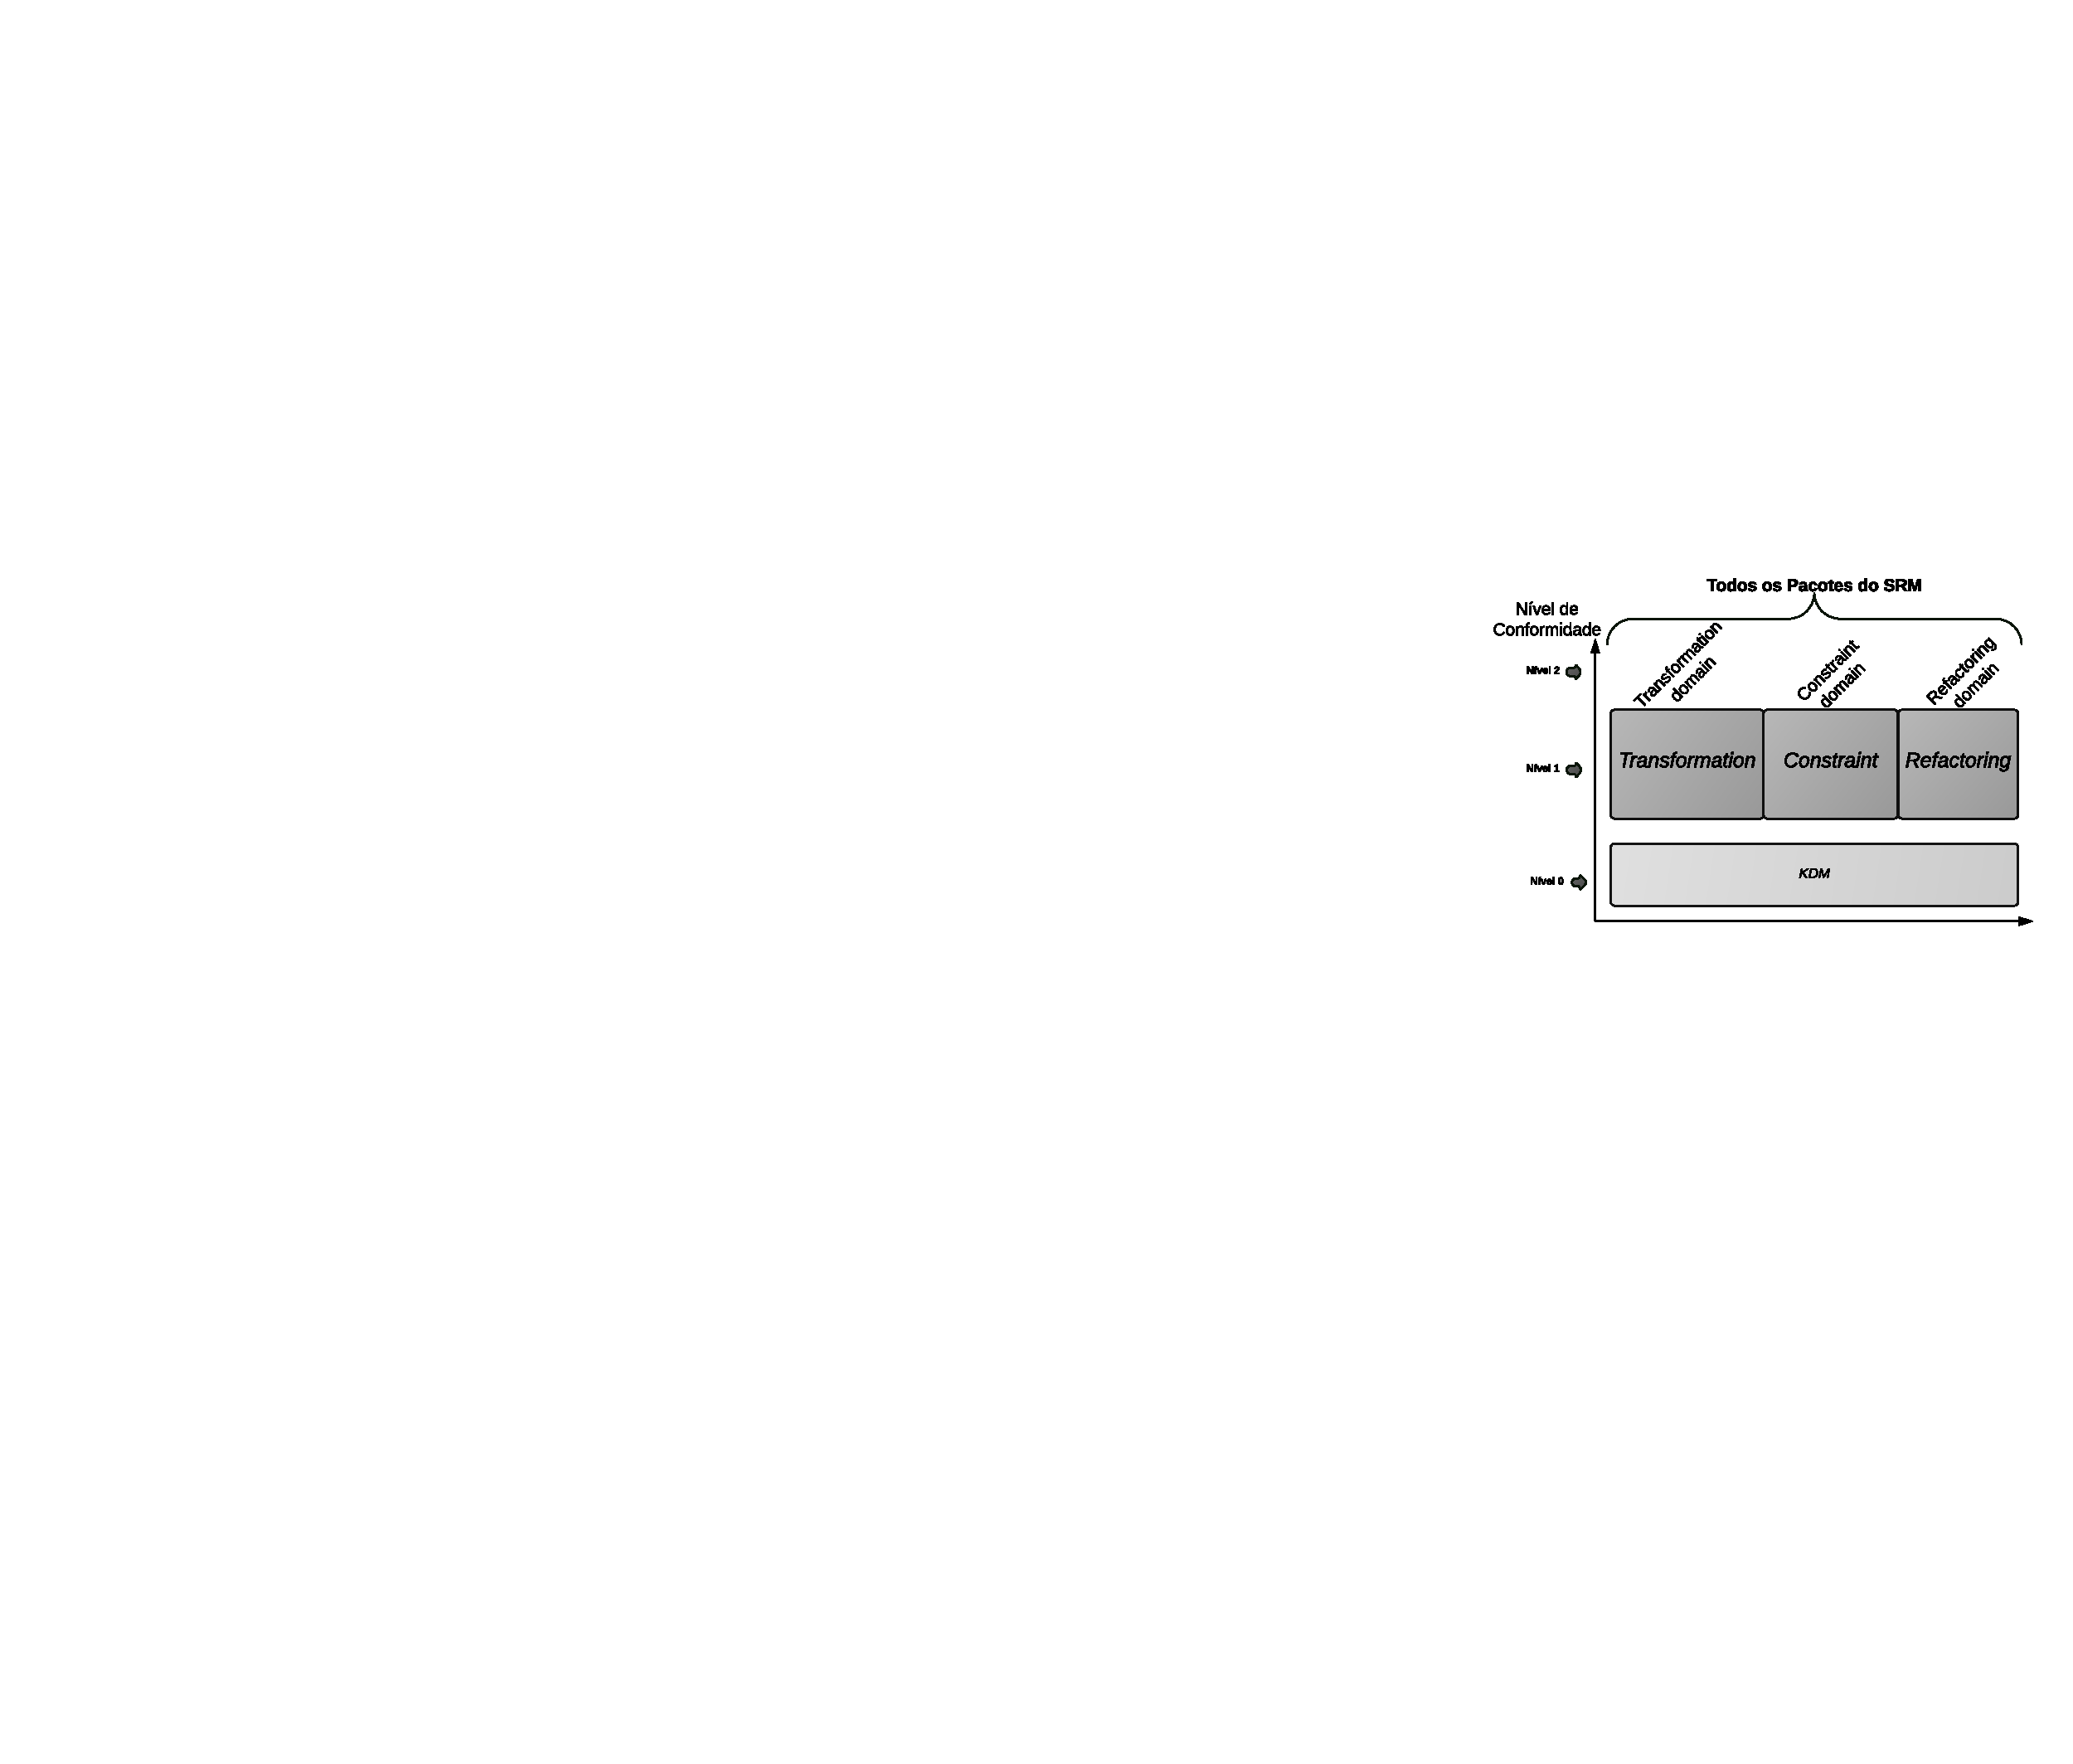
\includegraphics[scale=1]{images/pacotesSRM}
	\label{fig:pacotes_SRM_conformidade_level}
	\fautor
\end{figure}

\begin{itemize}
    \item \textbf{Nível 0}: nesse nível de conformidade são definidos os pacotes do KDM para representar os elementos estruturais que serão refatorados. Esse nível de conformidade representa um denominador comum que pode servir como uma base para a interoperabilidade entre diferentes categorias de ferramentas que utilizem o metamodelo SRM. Para que uma ferramenta esteja em conformidade com o \textbf{Nível 0} ela deve fornecer completo suporte para todas as metaclasses que foram definidas no KDM;
    \item \textbf{Nível 1}: nesse nível os pacotes definidos no \textbf{Nível 0} são utilizados para representar os elementos estruturais de uma refatoração. Esse nível define os seguintes pacotes: (\textit{i}) \texttt{Transformation}, (\textit{ii}) \texttt{Constraint} e (\textit{iii}) \texttt{Refactoring}. Para que uma ferramenta esteja em conformidade com o \textbf{Nível 1} ela deve fornecer suporte para todos os pacotes do \textbf{Nível 0} e pelo menos um dos pacotes do \textbf{Nível 1};
    \item \textbf{Nível 2}: esse nível é a união de todos os pacotes definidos no nível anterior. Para que uma ferramenta esteja em conformidade com o \textbf{Nível 2} ela deve fornecer suporte para todos os pacotes dos \textbf{Nível 0} e \textbf{Nível 1}.
\end{itemize}

Todos os pacotes do metamodelo SRM apresentados na Figura~\ref{fig:pacotes_SRM_conformidade_level} foram projetados e organizados esquematicamente em três camadas de abstração. As camadas de abstração são: (\textit{i}) \sigla{CEE}{Camada de Elementos Estruturais}, (\textit{ii}) \sigla{CR}{Camada de Refatoração} e (\textit{iii}) \sigla{CRTR}{Camada de Recurso de Transformação e Restrições}. As três camadas estão apresentadas na Figura~\ref{fig:camadas_e_pacotes_do_srm}.

\begin{figure}[h]
	\centering
	% Requires \usepackage{graphicx}
		\caption{Camadas e pacotes do SRM.}
	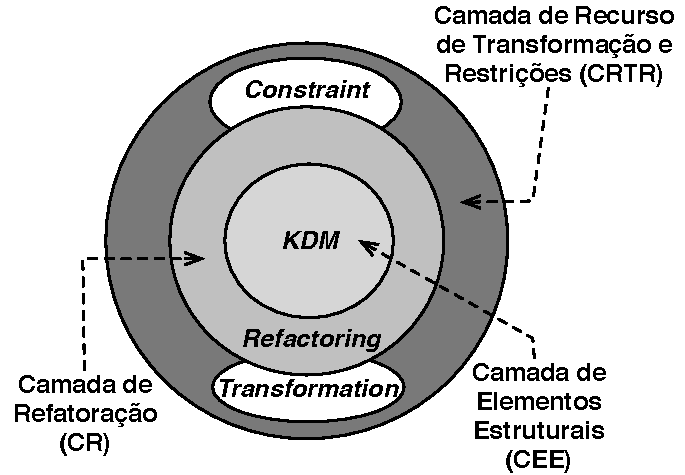
\includegraphics[scale=0.77]{images/LayerSRM}
	\label{fig:camadas_e_pacotes_do_srm}
	\fautor
\end{figure}

A camada CEE utiliza as metaclasses do metamodelo KDM para representar os elementos estruturais que serão refatorados. A camada CR contém o pacote \texttt{Refactoring}. Esse pacote define metaclasses para representar metadados sobre refatorações, tais como autor da refatoração, nome da refatoração, parâmetro, catálogo, etc. A camada CRTR contém dois pacotes: (\textit{i})  \texttt{Transformation} e \texttt{Constraint}. Coletivamente esses pacotes representam a operação/mecanismos e as restrições/asserções de uma determinada refatoração. A seguir os pacotes do SRM, bem como suas metaclasses são apresentados.

\subsubsection{Pacote \texttt{Refactoring}}

O pacote \texttt{Refactoring} define um conjunto de metaclasses cujo propósito é representar metadados de refatoração em alto nível. O pacote inclui metaclasses para definir a qual catálogo uma determinada refatoração pertence, definir o nome da refatoração, sua motivação, autor, parâmetros, classificação e sua biblioteca de refatoração, etc. Na Figura~\ref{fig:pacote_refactoring_srm} o pacote \texttt{Refactoring} e seus elementos (nove metaclasses e uma enumeração) são apresentados. Como ilustrado nesse figura o pacote \texttt{Refactoring} utiliza outras metaclasses que são definidas em outros pacotes: (\textit{i}) pacotes do KDM, (\textit{ii}) pacote \texttt{Transformation} e (\textit{iii}) pacote \texttt{Constraint}. Por exemplo, a operação de uma determinada refatoração é definida no pacote \texttt{Transformation}. Similarmente, as asserções de uma determinada refatoração são especificadas no pacote \texttt{Constraint}. Descrições sobre as metaclasses do pacote \texttt{Refactoring} são apresentas a seguir: 

\begin{figure}[h]
	\centering
	% Requires \usepackage{graphicx}
		\caption{Pacote \texttt{Refactoring} do SR.}
	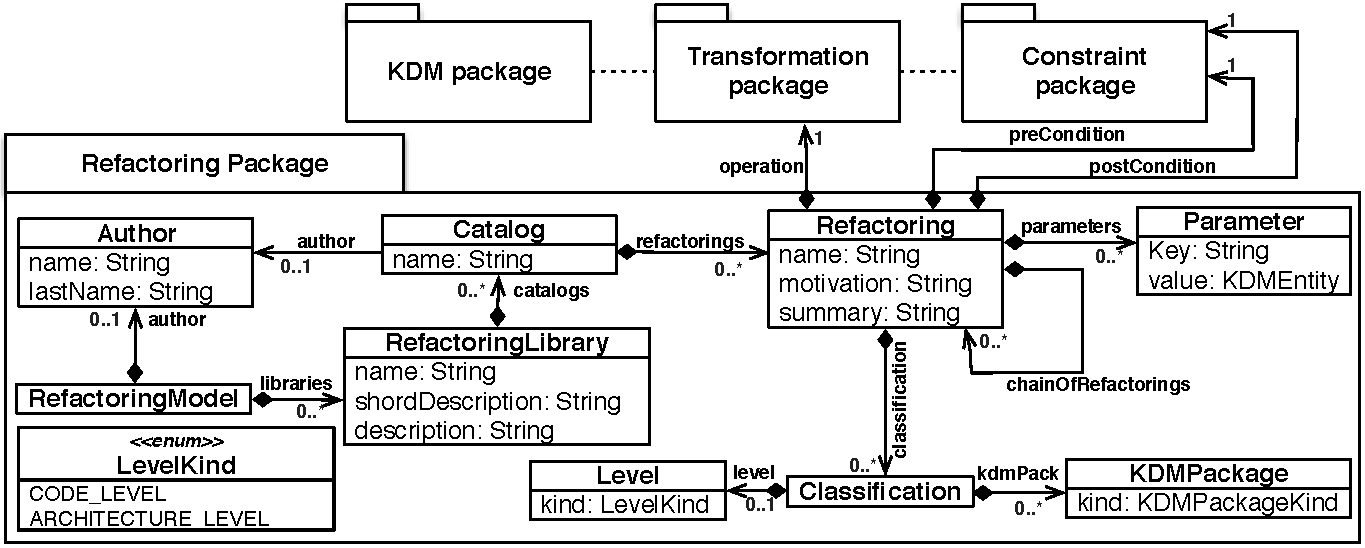
\includegraphics[scale=0.70]{images/pacoteRefactoring2}
	\label{fig:pacote_refactoring_srm}
	\fautor
\end{figure}

\begin{itemize}
\item \texttt{RefactoringModel} representa a metaclasse raiz do metamodelo. Essa metaclasse representa uma coleção de metadados que corresponde a uma ou mais refatorações definidas para o metamodelo KDM.

\begin{itemize}
	\item \textbf{Meta-associações}
		\begin{itemize}
			\item \texttt{author:Author[0..1]}: representa o autor de uma refatoração; 
			\item \texttt{libraries:RefactoringLibrary[0..*]}: representa um conjunto de biblioteca de refatorações que uma instância da metaclasse \texttt{RefactoringModel} possui..
		\end{itemize}
\end{itemize}

\item \texttt{Author} representa o autor de uma refatoração. Essa metaclasse contém dois meta-atributos.

\begin{itemize}
	\item \textbf{Meta-atributos}
		\begin{itemize}
			\item \texttt{name:String}: utilizado para definir o nome do autor;
			\item \texttt{lastName:String}: utilizado para definir o sobrenome do autor.
		\end{itemize}	
\end{itemize} 

\item \texttt{RefactoringLibrary} utilizado para descrever uma biblioteca de refatorações.

\begin{itemize}
	\item \textbf{Meta-atributos}
		\begin{itemize}
			\item \texttt{name:String}: utilizado para descrever o nome da biblioteca de refatoração;
			\item \texttt{shortDescription:String}: representa uma breve descrição sobre a biblioteca de refatoração;
			\item \texttt{description:String}: representa uma completa descrição sobre a biblioteca de refatoração.
		\end{itemize}	
\end{itemize} 

\begin{itemize}
	\item \textbf{Meta-associação}
		\begin{itemize}
			\item \texttt{catalogs:Catalog[0..*]}: um conjunto de catálogos que contem refatorações.
		\end{itemize}	
\end{itemize} 

\item \texttt{Catalog} metaclasse utilizada para representar um catalogo de refatorações.

\begin{itemize}
	\item \textbf{Meta-atributos}
		\begin{itemize}
			\item \texttt{name:String}: representa o nome do catálogo. 
		\end{itemize}	
\end{itemize} 

\begin{itemize}
	\item \textbf{Meta-associações}
		\begin{itemize}
			\item \texttt{author:Author[0..1]}: representa o autor do catalogo;
			\item \texttt{refactorings:Refactoring[0..*]}: conjunto de todas as refatorações que um catalogo possui.
		\end{itemize}	
\end{itemize} 

\item \texttt{Refactoring} representa uma das principais metaclasses do SRM.

\begin{itemize}
	\item \textbf{Meta-atributos}
		\begin{itemize}
			\item \texttt{name:String}: utilizado para identificar a refatoração e ajuda a construir um vocabulário comum para os desenvolvedores de software;
			\item \texttt{motivation:String}: descreve o motivo pelo qual a refatoração deve ser realizada – lista também as circunstâncias na qual a refatoração deve ser utilizada;
			\item \texttt{summary:String}: informa quando e onde uma determinada refatoração deve ser utilizada. Também é útil para auxiliar o engenheiro de software a identificar uma refatoração relevante em uma determinada situação. 
		\end{itemize}	
\end{itemize} 

\begin{itemize}
	\item \textbf{Meta-associações}
		\begin{itemize}
			\item \texttt{operation:Operation[1]}: representa a ação que será executa, ou seja, representa o mecanismo da refatoração;
			\item \texttt{preCondition:PreCondition[1]}: representa uma pré-condição que deve ser satisfeita antes da execução da operação/mecanismo da refatoração;
			\item \texttt{postCondition:PostCondition[1]}: representa uma pós-condição que tem como intuito verificar a corretude da refatoração;
			\item \texttt{parameters:Parameter[0..*]}: um conjunto de parâmetros que são utilizados para realizar a refatoração. Tais parâmetros podem ser metaclasses do KDM;
			\item \texttt{chainOfRefactoring:Refactoring[0..*]}: um conjunto de refatorações que quando combinadas descrevem uma refatoração mais complexas;
			\item \texttt{classification:Classification[0..*]}: define a classificação de uma refatoração.
		\end{itemize}	
\end{itemize} 

\item \texttt{Parameter} define um conjunto de parâmetros necessários para executar a refatoração. Essa metaclasse utiliza uma estrutura similar a tabela \textit{hash} para definir os parâmetros.

\begin{itemize}
	\item \textbf{Meta-atributos}
		\begin{itemize}
			\item \texttt{key:String}: representa o nome do parâmetro;
			\item \texttt{value:KDMEntity}: representa o tipo do parâmetro. Esse tipo deve ser metaclasses do metamodelo KDM.
		\end{itemize}	
\end{itemize} 

\item \texttt{Classification} define a classificação da refatoração.

\begin{itemize}
	\item \textbf{Meta-associações}
		\begin{itemize}
			\item \texttt{level}: representa se a refatoração é \textit{fine} ou \textit{macro grained refactoring};
			\item \texttt{kdmPack}: define qual pacote do KDM é necessário para executar a refatoração.
		\end{itemize}	
\end{itemize} 

\item \texttt{Level} utilizado para definir se a refatoração é de granularidade baixa ou alta.

\begin{itemize}
	\item \textbf{Meta-atributos}
		\begin{itemize}
			\item \texttt{kind:LevelKind}: especifica o level da refatoração.
		\end{itemize}	
\end{itemize} 

\item \texttt{KDMPackage} define qual pacote do KDM é necessário para executar a refatoração.

\begin{itemize}
	\item \textbf{Meta-atributos}
		\begin{itemize}
			\item \texttt{kind:KDMPackageKind}: representa qual pacote do KDM é necessário para executar a refatoração.
		\end{itemize}	
\end{itemize} 

\end{itemize}

\subsubsection{Pacote \texttt{Transformation}}

Conceitualmente, refatorações são definidas por meio de um conjunto de passos que devem ser seguidos para realizar uma determina mudança~\cite{Fowler1999, Demeyer1}. Por outro lado, programaticamente as refatorações são definidos como \aspas{programas} parametrizados que executam um conjunto de transformações seguindo uma ordem lógica. Usualmente, no contexto de modelos, tais transformações são conhecidas como endógenas e são implementadas utilizando técnicas de reescrita de grafo, ou como também é conhecida transformação de grafo (ver Capítulo~\ref{chapter:fundamentacao_teorica} Seção~\ref{sec:transformacoes_de_modelos}). Dessa forma, pode-se caracterizar que técnica de reescrita de grafo é útil para auxiliar na elaboração de transformações de forma independente para \textit{n} metamodelos, ou seja, técnica de reescrita de grafo pode ser aplicada em qualquer metamodelo que implemente o padrão MOF, como por exemplo o metamodelo KDM. Comumente, transformações em modelos são definidas utilizando linguagens específicas de transformações de modelos. Diversas linguagens de transformação de modelos têm sido propostas atualmente~\cite{Biehl_2010, Allilaire_06}, entre elas pode-se citar ATL e QVT.

Neste contexto, o pacote \texttt{Transformation} contém apenas uma metaclasse e uma enumeração para definir o mecanismo da refatoração. O propósito dessa metaclasse é representar metadados de ATL e/ou QVT. Com o uso da ATL e/ou QVT pode-se automatizar os mecanismos e todos os passos que uma determinada refatoração deve realizar. Dessa forma, com o propósito desse pacote é prover o reúso dos mecanismo e todos os passos de uma refatoração no contexto do metamodelo SRM, tanto ATL e QVT foram consideradas boas candidatas para especificar programaticamente os metadados sobre o mecanismo das refatorações. Por tanto, o SRM permite persistir metadados relacionados a ATL e QVT.

Na Figura~\ref{fig:pacote_transformation_srm} é mostrado esquematicamente o pacote \texttt{Transformation}, sua metaclasse e uma enumeração. Como ilustrado nessa figura o pacote \texttt{Transformation} utiliza outros pacotes: (\textit{i}) pacotes do KDM, (\textit{ii}) pacote \texttt{Refactoring} e (\textit{iii}) pacote \texttt{Constraint}. A seguir uma descrição de cada elemento desse pacote é apresentado.

\begin{figure}[h]
	\centering
	% Requires \usepackage{graphicx}
		\caption{Pacote \texttt{Transformation} do SRM.}
	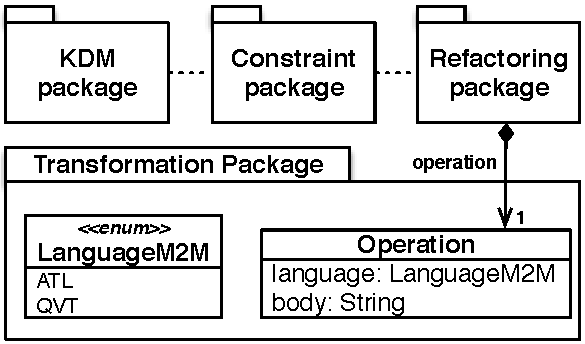
\includegraphics[scale=0.70]{images/TransformationPackageSRM4}
	\label{fig:pacote_transformation_srm}
	\fautor
\end{figure}

\begin{itemize}
    \item \texttt{Operation} também representa uma das principais metaclasses do SRM. Essa metaclasse possui metadados do código responsável por realizar a transformação/refatoração.

\begin{itemize}
	\item \textbf{Meta-atributos}
		\begin{itemize}
			\item \texttt{language:LanguageM2M}: especifica a linguagem que será escrito o código responsável por realizar a transformação/refatoração. Valores válidos são: ``ATL'' e ``QVT'';
			\item \texttt{body:String}: especifica a transformação/refatoração com base na linguagem selecionada, ``ATL'' ou ``QVT''.
		\end{itemize}	
\end{itemize}
     
     \item \texttt{LanguageM2M}: representa quais os tipos de linguagens de transformação de modelos podem ser utilizadas para implementar a refatoração. Os valores possíveis são: \aspas{ATL} ou \aspas{QVT};
     
\end{itemize}

\subsubsection{Pacote \texttt{Constraint}}

É importante que o metamodelo SRM permita definir asserções e não apenas o mecanismo da refatoração, assim, engenheiros podem utilizar uma determinada instância do metamodelo SRM e verificar quais são as asserções que eles devem respeitar para executar a refatoração de forma correta. Tais asserções no contexto de refatorações são conhecidas como pré- e pós-condições~\cite{OPDYKE_1992, Roberts_1999}. Asserções são úteis para garantir que a sintaxe e semântica do modelo sejam preservadas após a aplicação das refatorações, assegurando assim uma possível preservação de comportamento.

Neste contexto o pacote \texttt{Constraint} do SRM contém três metaclasses e uma enumeração para definir as asserções (pré- e pós-condições) de uma determinada refatoração. O propósito desse pacote é representar metadados sobre asserções utilizando as linguagens OCL e/ou XQuery. Utilizando essas linguagens, é possível verificar, por exemplo, se todos os parâmetros obrigatórios para executar uma refatoração foram especificados corretamente. Assegurar que a refatoração será aplicada de forma correta é de suma importância para preservar a sintaxe e semântica da instância do metamodelo, como por exemplo, preservar comportamentos. Na Figura~\ref{fig:pacote_constraint_srm} é mostrado o pacote \texttt{Constraint}, suas metaclasses e uma enumeração. A seguir os elementos desse pacote são descritos:

\begin{figure}[h]
	\centering
	% Requires \usepackage{graphicx}
		\caption{Pacote \texttt{Constraint} do SRM.}
	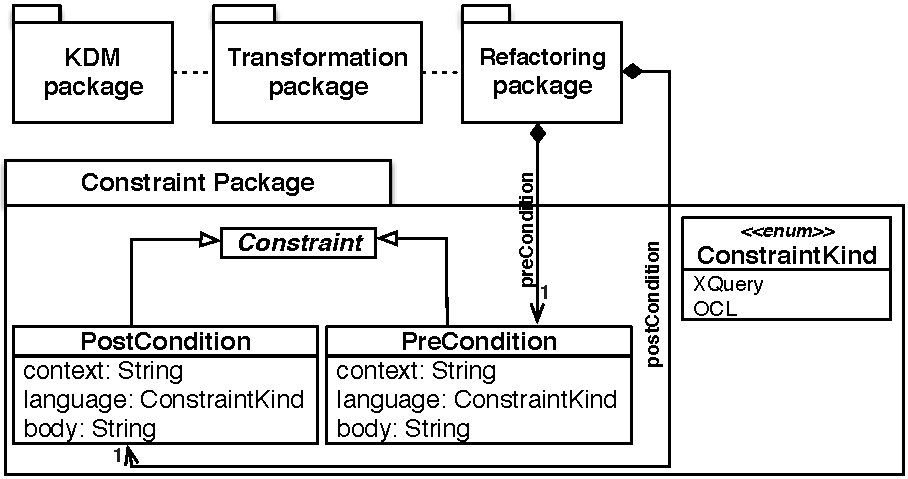
\includegraphics[scale=0.70]{images/pacoteConstraint3}
	\label{fig:pacote_constraint_srm}
	\fautor
\end{figure}

\begin{itemize}
    
    \item \texttt{Constraint} representa a metaclasse raiz de asserções. Em outras palavras, essa metaclasse representa de forma genérica que todas as refatorações possuem asserções/restrições. Essa metaclasse é abstrata e não é instanciada.
    
    \item \texttt{PreCondition} define uma pré-condição para ser executada antes de operação/refatoração.

\begin{itemize}
	\item \textbf{Meta-atributos}
		\begin{itemize}
			\item \texttt{context:String}: especifica o classificador para qual a pré-condição será definido;
			\item \texttt{language:ConstraintKind}: especifica a linguagem que será escrito a pré-condição. Valor válido é: ``OCL'' ou ``XQuery'';
			\item \texttt{body:String}: especifica a OCL ou ``XQuery'' que representa a pré-condição.
		\end{itemize}	
\end{itemize} 

\item \texttt{PostCondition} define uma pós-condição para ser executada após a operação/refatoração.

\begin{itemize}
	\item \textbf{Meta-atributos}
		\begin{itemize}
			\item \texttt{context:String}: especifica o classificador para qual a pós-condição será definido;
			\item \texttt{language:ConstraintKind}: especifica a linguagem que será escrito a pós-condição. Valor válido é: ``OCL'' ou ``XQuery'';
			\item \texttt{body:String}: especifica a OCL ou ``XQuery'' que representa a pós-condição.
		\end{itemize}	
\end{itemize}

\item \texttt{ConstraintKind}: representa quais os tipos de linguagens de restrições de modelos podem ser utilizadas para implementar a asserção. Os valores possíveis são: \aspas{OCL} ou \aspas{XQuery};
    
\end{itemize}

%Para facilitar o entendimento do metamodelo SRM, bem como o relacionamento entre suas metaclasses a seguir são apresentadas descrições de como cada metaclasse se relacionam e devem ser utilizadas para proporcionar o reúso de refatorações para o metamodelo KDM.

%\subsection{Metaclasses \texttt{RefactoringModel}, \texttt{Author} e \texttt{RefactoringLibrary} }

%\texttt{RefactoringModel} representa a metaclasse raiz do metamodelo SRM. Em outras palavras, essa metaclasse representa uma coleção de metadados que corresponde a uma ou mais refatorações definidas para o metamodelo KDM. Essa metaclasse não contém nenhum meta-atributo, porém, como apresentado anteriormente possui duas associações: (\textit{i}) \texttt{author:Author[0..1]} e (\textit{ii}) \texttt{libraries:RefactoringLibrary[0..*]}

\subsection{Implementar o SRM}\label{sec:implementacao_do_SRM}

A junção dos pacotes apresentados nas seções anteriores e suas metaclasses formam o metamodelo SRM. Na Figura~\ref{fig:meta_modelo_SRM} é apresentado esquematicamente o metamodelo SRM. Como pode ser observado o SRM contém 13 metaclasses e quatro enumerações. O metamodelo SRM foi implementado utilizando EMF.

\begin{figure}[h]
	\centering
	% Requires \usepackage{graphicx}
	\caption{Visão de árvore do SRM implementado em EMF.}
	\label{fig:visao_arvore_srm_emf}
	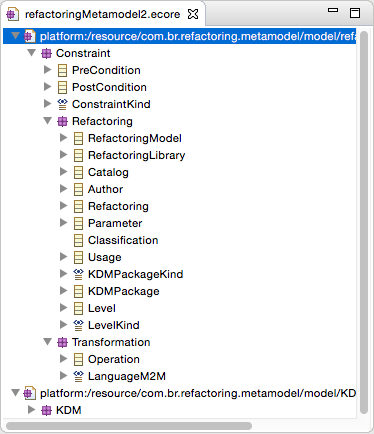
\includegraphics[scale=0.65]{images/srm_emf}
	\fautor
\end{figure}

Na Figura~\ref{fig:visao_arvore_srm_emf} é possível ver o SRM implementado em EMF. Todos os pacotes do metamodelo SRM contém internamente um conjunto de metaclasses. Da mesma forma, cada metaclasse contém seus meta-atributos e seus tipos.

\section{Gramática da DSL utilizada para instanciar o SRM}

Como já salientado o SRM foi implementado utilizando o EMF. Dessa forma, existem duas opções para instanciar o metamodelo SRM: (\textit{i}) utilizando uma visão de árvore do metamodelo e (\textit{ii}) utilizando a API fornecida pelo EMF. A primeira opção, utiliza uma visão de árvore da instância do metamodelo SRM, como apresentado na Figura~\ref{fig:visao_arvore_metamodelo_srm}. Quando o engenheiro de modernização clica com o botão direito metaclasses do metamodelo são apresentadas para que o engenheiro escolha qual metaclasse especificar e instanciar. Porém, note que o engenheiro de modernização deve conhecer a estrutura correta do metamodelo SRM para utilizar a visão de árvore. 

\begin{figure}[h]
	\centering
	% Requires \usepackage{graphicx}
	\caption{Visão de árvore de uma instância do metamodelo SRM.}
	\label{fig:visao_arvore_metamodelo_srm}
	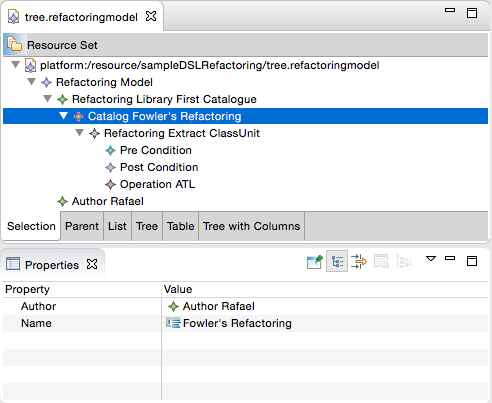
\includegraphics[scale=0.65]{images/tree_srm}
	\fautor
\end{figure}

A segunda opção é a utilização da API fornecida pelo EMF. Nesta segunda opção a linguagem Java é utilizada juntamente com a API EMF. Para utilizar a segunda opção os engenheiros de modernização necessitam ter conhecimento avançado de Java, isto é, a instanciação de uma refatoração utilizando a segunda opção é bastante verbosa, complexa e propensa a erros, pois exige conhecimento avançadas de refatoração e habilidades de programação em relação a API Ecore/EMF. 

No Código-fonte~\ref{cod:instancia_do_SRM} é apresentado um trecho onde é feita a instanciação em memória de algumas metaclasses definidas no metamodelo SRM utilizando a segunda opção. Note que nesse código-fonte a instanciação das metaclasses do metamodelo SRM é um processo verboso e propenso a erros. Para instanciar o metamodelo SRM o engenheiro deve saber utilizar a API do \textit{framework} EMF. Metaclasses são instanciadas em EMF utilizando o conceito de fabrica (em inglês - \textit{Factory}). Cada fabrica de uma metaclasse possui um método \texttt{createX}, onde X representa o nome da metaclasse do metamodelo. 

Para criar uma instancia válida do metamodelo SRM o engenheiro de modernização deve seguir um conjunto de passos. Por exemplo, como pode ser observado na linha 1 do Código-fonte~\ref{cod:instancia_do_SRM} uma instância da metaclasse \texttt{Author} é criada por meio da interface \texttt{RefactoringModelFactory} e do método \texttt{createAuthor()}. Em seguida, todos os meta-atributos da metaclasse \texttt{Author} devem ser especificados como apresentado nas linhas 2 e 3 do Código-fonte~\ref{cod:instancia_do_SRM}. Nas linhas 4-14 outras metaclasses do metamodelo SRM são instanciadas. 

\begin{codigo}[caption={[Instanciação do metamodelo SRM programaticamente.] Instanciação do metamodelo SRM.},escapeinside={(*@}{@*)}, basicstyle=\footnotesize, label={cod:instancia_do_SRM}, language=Java]{Name}
Author author = RefactoringModelFactory.eINSTANCE.createAuthor();
author.setName("Rafael");
author.setLastName("Durelli");
RefactoringModel rM = RefactoringModelFactory.eINSTANCE.createRefactoringModel();
rM.setAuthor(author);
RefactoringLibrary library = RefactoringModelFactory.eINSTANCE.createRefactoringLibrary();
lib.setName("Fowler's refactorings");
lib.setDescription("Contains some Fowler's refactorings such as ExtractClass, RenameElements, PushMethod, PushAttribute, etc.");
lib.setShortDescription("Fine grained Refactorings");
rM.getLibraries().add(lib);
Catalog cat = RefactoringModelFactory.eINSTANCE.createCatalog();
cat.setAuthor(author);
cat.setName("Fowler's catalog");
libr.getCatalogs().add(cat);
...
\end{codigo}

Como observado o processo de instanciação do metamodelo SRM não é um processo trivial em ambas opções. Além disso, engenheiros de modernização devem estar familiarizados como as semânticas das refatorações (por exemplo, qual(is) é (são) o(s) pré-requisito(s) para a execução de uma refatoração) e como/onde utilizar e programar tais refatorações. Com o intuito de facilitar e diminuir a quantidade de código-fonte, esforço obrigatórios e competência necessárias para instanciar refatorações utilizando o metamodelo SRM, foi criado uma DSL para auxiliar a instanciação de refatorações. A seguir as gramáticas definidas que regem a DSL para auxiliar a instanciação do metamodelo SRM são apresentadas.

%
%Cada trecho de código da DSL representa uma instancia de uma metaclasse do metamodelo SRM, ou seja, cada declaração da DSL está em conformidade com uma metaclasse do SRM. Por exemplo, considere a palavra-chave \texttt{refactoringModel} \texttt{author} entre \aspas{\{} e \aspas{\}} representa a instanciação da metaclasse \texttt{Author} do SRM que possui dois meta-atributos: \texttt{name} e \texttt{lastName}. 
%
A DSL criada para auxiliar a instanciação do SRM foi desenvolvida utilizando Xtext\footnote{\texttt{https://www.eclipse.org/Xtext/}}. Xtext é um \textit{framework} do Eclipse\footnote{\texttt{https://www.eclipse.org}} que tem como principal objetivo automatizar e agilizar o processo de desenvolvimento de DSLs. %Note que a sintaxe da DSL segue as terminologias e conceitos definidos no metamodelo SRM para facilitar a utilização da DSL e o entendimento do metamodelo SRM.

Em Xtext a gramática segue uma notação similar ao \textit{Backus–Naur Form} (BNF) chamada de regras do \textit{parser}. Tais regras representam a sintaxe concreta da DSL. Note que para facilitar o entendimento da DSL, trechos da mesma são mostradas em listagens de códigos separados, bem como símbolos para explanar o propósito de uma terminada linha da gramática. No Código-fonte~\ref{lst:dsl_part_1} é ilustrado o primeiro trecho da gramática concreta da DSL desenvolvida. A gramática começa com a definição do nome da DSL (SRM) (ver Código-fonte~\ref{lst:dsl_part_1} \ding{182}). Em sequência é definido os metamodelos que devem ser importados para serem utilizados durante a criação da DSL: o metamodelo SRM\ding{183} e o Ecore\ding{184}.


\begin{lstlisting}[language=Xtext, frame=single, basicstyle={\scriptsize}, mathescape=true, label={lst:dsl_part_1}, caption={Gramática da DSL - parte 1}]
$\textrm{\ding{182}}$ grammar refactoring.xtext.SRM with org.eclipse.xtext.common.Terminals 
$\textrm{\ding{183}}$ import platform:/resource/refactoring/model/SRM.ecore
$\textrm{\ding{184}}$ import http://www.eclipse.org/emf/2002/Ecore as ecore
RefactoringModel: 
	$\textrm{\ding{185}}$ `refactoringModel' name = ID `{'
	$\textrm{\ding{186}}$ author = Author
	$\textrm{\ding{187}}$ libraries += RefactoringLibrary$^{*}$;
	`}'
\end{lstlisting}


Em seguida é criado a primeira regra. Essa regra começa com a definição da metaclasse \texttt{RefactoringModel}. O corpo da regra começa logo após os \aspas{\texttt{:}}. Primeiramente para o entendimento da regra, é importante destacar que literais de \textit{string} (em Xtext os literais podem ser expressos com aspas simples ou duplas) definem palavras-chave da DSL. Como pode ser observado no Código-fonte~\ref{lst:dsl_part_1} é esperado a palavra-chave \texttt{refactoringModel}\ding{185} seguido por um \texttt{ID} e \aspas{\{}. A gramática que rege o objeto \texttt{ID} é definida como uma sequência ilimitada de maiúsculas e minúsculas, números e o carácter de sublinhado, embora possa não começa por um dígito. A gramática que representa o nó \texttt{ID}\ding{182} pode ser visualizada no Código-fonte~\ref{lst:dsl_part_2}. 

\begin{lstlisting}[language=Xtext, frame=single, basicstyle=\scriptsize, mathescape=true, label={lst:dsl_part_2}, caption={Gramática da DSL - parte 2}]
	$\textrm{\ding{182}}$ terminal ID: (`a'..`z' | `A'..`Z'|`_')(`a'..`z' | `A'..`Z'|`_'|`0'..`9')*;
\end{lstlisting}

Ainda no Código-fonte~\ref{lst:dsl_part_1} a expressão \texttt{author=Author}\ding{186} especifica que pode-se instanciar uma instancia da metaclasse \texttt{Author}. A expressão \texttt{(libraries += RefactoringLibrary)$^{*}$}\ding{187} descrita no Código-fonte~\ref{lst:dsl_part_1} especifica que pode-se instanciar várias instâncias da metaclasse \texttt{RefactoringLibrary}. O operador estrela, \aspas{\texttt{*}}, ilustra que o número de elementos (nesse caso \texttt{RefactoringLibrary}) é arbitrário; em particular, ele pode ser qualquer número \texttt{>=} 0. Operador \texttt{+=} por sua vez representa que a propriedade \texttt{libraries} será uma lista do tipo \texttt{RefactoringLibrary}.

\begin{lstlisting}[language=Xtext, frame=single, basicstyle=\scriptsize, mathescape=true, label={lst:dsl_part_3}, caption={Gramática da DSL - parte 3}]
Author:
	$\textrm{\ding{182}}$ `author' `{'
	$\textrm{\ding{183}}$ `name' `:' name = ID  
		$\textrm{\ding{229} \ding{184}}$ `lastName' `:' lastName = ID; 
`}'
RefactoringLibrary:
	$\textrm{\ding{185}}$ `refactoringLibraries' `{'
	$\textrm{\ding{186}}$ `name' `:' name = ID  
		$\textrm{\ding{229}}$ `shortDescription' `:' shortDescription = STRING
		$\textrm{\ding{229}}$ `description' `:' description = STRING
		$\textrm{\ding{229}}$ $\textrm{\ding{187}}$ catalogs += Catalog$^{*}$
`}'
\end{lstlisting}

A definição das regras que regem as metaclasses \texttt{Author} e \texttt{RefactoringLibrary} são apresentadas no Código-fonte~\ref{lst:dsl_part_3}. A regra para a definição de \texttt{Author} começa com a definição da palavra-chave \texttt{author} seguida por um \aspas{\{}\ding{182}. Em seguida a palavra-chave \texttt{name} é esperada, seguido por \aspas{\texttt{:}} \ding{183}. Posteriormente a palavra-chave \texttt{lastName} também é esperada, seguido por \aspas{\texttt{:}} \ding{184}. Na linha 6 do Código-fonte~\ref{lst:dsl_part_3} começa a definição da regra da metaclasse \texttt{RefactoringLibrary}. A regra para a definição de \texttt{RefactoringLibrary} começa com a definição da palavra-chave \texttt{refactoringLibraries} seguida por um \aspas{\{}\ding{185}. Em seguida, deve-se especificar a palavra-chave \texttt{name} e \texttt{:}. Posteriormente, as palavras-chaves \texttt{shortDescription} e \texttt{description} são especificadas nas linhas 9 e 10, respectivamente. A expressão descrita na Linha 11 representa que pode haver qualquer número de instâncias da metaclasse \texttt{Catalog}.

\begin{lstlisting}[language=Xtext, frame=single, basicstyle=\scriptsize, mathescape=true, label={lst:dsl_part_4}, caption={Gramática da DSL - parte 4}]
Catalog:
	$\textrm{\ding{182}}$`catalog' `{' 
		$\textrm{\ding{229} \ding{183}}$`name' `:' name=ID
		$\textrm{\ding{229} \ding{184}}$`author' `:' author=[Author]
		$\textrm{\ding{229} \ding{185}}$refactorings += Refactoring$^{*}$
	`}'
Refactoring:
	`refactoring' `{' 
		$\textrm{\ding{229}}$`name' `:' name = ID
		$\textrm{\ding{229}}$`motivation' `:' motivation = STRING
		$\textrm{\ding{229}}$`summary' `:' summary = STRING
		$\textrm{\ding{229} \ding{186}}$ operation = Operation?
		$\textrm{\ding{229} \ding{187}}$ preCondition = PreCondition?
		$\textrm{\ding{229} \ding{188}}$ postCondition = PostCondition?
		$\textrm{\ding{229} \ding{190}}$(`containedRefactoring' `:' chainOfRefactoring+=Refactoring)$^{*}$
	`}'
\end{lstlisting}

O Código-fonte~\ref{lst:dsl_part_4} representa as sintaxes concretas das metaclasses \texttt{Catalog} e \texttt{Refactoring}. A sintaxe concreta da metaclasse \texttt{Catalog} começa com a palavra-chave \texttt{catalog} seguida por um \aspas{\{}\ding{182}. Em seguida o nome do catálogo de refatoração deve ser especifica por meio da palavra-chave \texttt{name} \ding{183}. Posteriormente, deve-se especificar uma instância da metaclasse \texttt{Author}, informando quem é o autor desse catalogo de refatoração, ver Código-fonte~\ref{lst:dsl_part_4}\ding{184}. Na Linha 5 do Código-fonte~\ref{lst:dsl_part_4} deve-se informar várias instâncias da metaclasse \texttt{Refactoring}, essa sintaxe representa as refatorações que compõem esse catalogo de refatoração. Nas linhas 7-16 a definição da sintaxe concreta para a definição de uma refatoração por meio do metamodelo SRM é apresentada. Inicialmente, uma refatoração deve possuir um nome, conforme ilustrado na linha 9 do Código-fonte~\ref{lst:dsl_part_4}. Posteriormente, a motivação, bem como o resumo da refatoração também devem ser especificados, conforme apresentado nas linhas 10 e 11 do Código-fonte~\ref{lst:dsl_part_4}. As linhas 12, 13, 14 e 15 informam que uma metaclasse do tipo \texttt{Operation}\ding{186}, \texttt{PreCondition}\ding{187} e \texttt{PostCondition}\ding{188} devem ser instanciadas, respectivamente. Na linha 15 representa a sintaxe da DSL para especificar um conjunto de refatorações que quando combinadas podem realizar refatorações complexas.

\begin{lstlisting}[language=Xtext, frame=single, basicstyle=\scriptsize, mathescape=true, label={lst:dsl_part_5}, caption={Gramática da DSL - parte 5}]
Operation: 
	$\textrm{\ding{182}}$`operation' `{'
		$\textrm{\ding{229}}$`language' `:' language=LanguageM2M
		`body' `:' `{'
			$\textrm{\ding{229} \ding{184}}$body = STRING
		`}'
	`}'
PreCondition: 
	$\textrm{\ding{185}}$`preCondition' `{'
		$\textrm{\ding{229}}$`context' `:' context=STRING
		$\textrm{\ding{229}}$`language' `:' language=ConstraintKind
		`body' `:' `{' 
			$\textrm{\ding{229}}$body=STRING	
		`}'
	`}'
PostCondition: 
	$\textrm{\ding{186}}$`postCondition' `{'
		$\textrm{\ding{229}}$`context' `:' context=STRING
		$\textrm{\ding{229}}$`language' `:' language=ConstraintKind
		`body' `:' `{' 
			$\textrm{\ding{229}}$body=STRING	
		`}'
	`}'
enum LanguageM2M: 
	ATL | QVT
enum ConstraintKind: 
	XQuery | OCL

\end{lstlisting}

No Código-fonte~\ref{lst:dsl_part_5} as sintaxes concretas das metaclasses \texttt{Operation}, \texttt{PreCondition} e \texttt{PostCondition} são definidas. A sintaxe concreta da metaclasse \texttt{Operation} inicia com a palavra-chave \texttt{operation} seguida por um \aspas{\{}\ding{182}. Em seguida, deve-se especificar qual a linguagem que a operação/refatoração será escrita. \texttt{LanguageM2M} é uma enumeração (\textit{enum}) que está representado na linha 24 do Código-fonte~\ref{lst:dsl_part_5}. A linha 5 representa a sintaxe concreta para especificar o \aspas{corpo} da operação/refatoração propriamente dita \ding{184}. Na linha 8 a sintaxe concreta da metaclasse \texttt{PreCondition} é definida. A sintaxe concreta inicia com a palavra-chave \texttt{preCondition} seguida por um \aspas{\{}\ding{182}, \texttt{context}, \texttt{language} e \texttt{body}. A sintaxe concreta da metaclasse \texttt{PostCondition} é definida nas linhas 16 até 23. Note que a sintaxe é similar à sintaxe definida na metaclasse \texttt{PreCondition}. A partir das gramáticas da DSL apresentadas, XText gera um editor textual no ambiente de desenvolvimento Eclipse IDE. Esse editor textual provê \textit{highlighting} de sintaxe, \textit{code completion} e \textit{code navigation}. O editor resultante pode ser observado no Capítulo~\ref{chapter:ferramenta_kdm_re} na Seção~\ref{label:sec_modulo_do_srm}, onde é apresentada a ferramenta KDM-RE.

\subsection{Exemplo de uso da DSL}

A partir das gramáticas da DSL apresentadas o engenheiro de modernização pode instanciar o metamodelo SRM e prover o reuso de uma determinada refatoração. Nesta seção exemplos graduais são apresentados para facilitar o entendimento de como utilizar a DSL. Dessa forma, para ilustrar o uso da DSL nessa seção considere que o engenheiro de modernização almeja prover o reúso de uma determinada refatoração utilizando a DSL. Dessa forma, as regras que regem as gramáticas devem ser seguidas. De acordo com a gramática definida no Código-fonte~\ref{lst:dsl_part_1}, primeiro o engenheiro de modernização deve instanciar a metaclasse \texttt{RefactoringModel}. Isto é feito por meio da palavra-chave \texttt{refactoringModel} seguido por \{ e \} como apresentado no Código-fonte~\ref{cod:SRM_part1}.

\begin{codigo}[caption={[Exemplo de uso da DSL - parte 1.] Exemplo de uso da DSL - parte 1.},escapeinside={(*@}{@*)}, basicstyle=\footnotesize, label={cod:SRM_part1}, language=myDSL]{Name}
refactoringModel {

}
\end{codigo}

De acordo com a gramática (ver Código-fonte~\ref{lst:dsl_part_1}) o próximo passo é o engenheiro de modernização especificar o autor da refatoração. Isto é realizado por meio da palavra-chave \texttt{author} seguido por \{ e \}. Dentro do escopo da palavra-chave \texttt{author} deve-se especificar o nome e o sobrenome do autor como apresentado no Código-fonte~\ref{cod:SRM_part2}

\begin{codigo}[caption={[Exemplo de uso da DSL - parte 2.] Exemplo de uso da DSL - parte 2.},escapeinside={(*@}{@*)}, basicstyle=\footnotesize, label={cod:SRM_part2}, language=myDSL]{Name}
refactoringModel {
    author {
		name : Rafael
		lastName : Durelli
	}
}
\end{codigo}

Posteriormente deve-se instanciar a metaclasse \texttt{RefactoringLibrary} e seus meta-atributos. De acordo com a gramática da DSL isso é feito por meio da palavra-chave \texttt{refactoring\-Libraries} seguido por \{ e \}, ver linha 6 do Código-fonte~\ref{cod:SRM_part3}. 

\begin{codigo}[caption={[Exemplo de uso da DSL - parte 3.] Exemplo de uso da DSL - parte 3.},escapeinside={(*@}{@*)}, basicstyle=\footnotesize, label={cod:SRM_part3}, language=myDSL]{Name}
refactoringModel {
    author {
		name : Rafael
		lastName : Durelli
	}
	refactoringLibraries {
	    name : FineGrainedRefactoring
		shortDescription : "contains a set of refactorings"
		description : "refactorings"
	}
}
\end{codigo}

Em seguida deve-se instanciar a metaclasse \texttt{Catalog}. De acordo com a gramática apresentada no Código-fonte~\ref{lst:dsl_part_4} isso é feito por meio da palavra-chave \texttt{catalog} seguido por \{ e \} ver linhas 10-12 do Código-fonte~\ref{cod:SRM_part4}.

\begin{codigo}[caption={[Exemplo de uso da DSL - parte 4.] Exemplo de uso da DSL - parte 4.},escapeinside={(*@}{@*)}, basicstyle=\footnotesize, label={cod:SRM_part4}, language=myDSL]{Name}
refactoringModel {
    author {
		name : Rafael
		lastName : Durelli
	}
	refactoringLibraries {
	    name : FineGrainedRefactoring
		shortDescription : "contains a set of refactorings"
		description : "refactorings"
		catalog {
			name : Fowler Catalog
			author : Rafael
		}
	}
}
\end{codigo}

Cada catálogo de refatoração contém um conjunto de refatorações. Dessa forma, o próximo passo é realizar a instanciação da metaclasse \texttt{Refactoring} e seus meta-atributos. Isto pode ser realizado por meio da palavra-chave \texttt{refactoring} seguido por \{ e \} como apresentado na gramática da DSl (ver Código-fonte~\ref{lst:dsl_part_4}).

\begin{codigo}[caption={[Exemplo de uso da DSL - parte 5.] Exemplo de uso da DSL - parte 5.},escapeinside={(*@}{@*)}, basicstyle=\footnotesize, label={cod:SRM_part5}, language=myDSL]{Name}
refactoringModel {
    author {
		name : Rafael
		lastName : Durelli
	}
	refactoringLibraries {
	    name : FineGrainedRefactoring
		shortDescription : "contains a set of refactorings"
		description : "refactorings"
		catalog {
			name : Fowler Catalog
			author : Rafael
			refactoring {
				name : Create a class
				motivation : "A new class is needed"
				summary : "A new class is created in a package"
			}
		}
	}
}
\end{codigo}

Como observado no Código-fonte~\ref{cod:SRM_part5} a metaclasse \texttt{Refactoring} é instanciada nas linhas 13-16. Assim, seus meta-atributos também devem ser informados, ou seja, \texttt{name}, \texttt{motivation} e \texttt{summary}. Após instanciar a metaclasse \texttt{Refactoring} o próximo passo é instanciar a metaclasse \texttt{Operation} como apresentado no Código-fonte~\ref{cod:SRM_part6} linhas 17-21. Note que para facilitar o entendimento da DSL o código em ATL (ver linhas 19-21) que representa a operação da refatoração foi removido.

\begin{codigo}[caption={[Exemplo de uso da DSL - parte 6.] Exemplo de uso da DSL - parte 6.},escapeinside={(*@}{@*)}, basicstyle=\footnotesize, label={cod:SRM_part6}, language=myDSL]{Name}
refactoringModel {
    author {
		name : Rafael
		lastName : Durelli
	}
	refactoringLibraries {
	    name : FineGrainedRefactoring
		shortDescription : "contains a set of refactorings"
		description : "refactorings"
		catalog {
			name : Fowler Catalog
			author : Rafael
			refactoring {
				name : Create a class
				motivation : "A new class is needed"
				summary : "A new class is created in a package"
				operation {
				    language : ATL
				    body : {
				        TO BE DEFINED
				    }
				}
			}
		}
	}
}
\end{codigo}

\begin{codigo}[caption={[Exemplo de uso da DSL - parte 7.] Exemplo de uso da DSL - parte 7.},escapeinside={(*@}{@*)}, basicstyle=\footnotesize, label={cod:SRM_part7}, language=myDSL]{Name}
refactoringModel {
    author {
		name : Rafael
		lastName : Durelli
	}
	refactoringLibraries {
	    name : FineGrainedRefactoring
		shortDescription : "contains a set of refactorings"
		description : "refactorings"
		catalog {
			name : Fowler Catalog
			author : Rafael
			refactoring {
				name : Create a class
				motivation : "A new class is needed"
				summary : "A new class is created in a package"
				operation {
				    language : ATL
				    body : {
				        TO BE DEFINED
				    }
				}
				preCondition {
					context : ClassUnit
					language : OCL
					body : {
						"TO BE DEFINED"
					}
			    }
			    postCondition {
					context : ClassUnit
					language : OCL
					body : {
						"TO BE DEFINED"
					}
				}
		}
	}
}
\end{codigo}

Como apresentado na gramática da DSL (ver Código-fonte~\ref{lst:dsl_part_4}) após instanciar a metaclasse \texttt{Operation} deve-se instanciar as asserções, ou seja, instanciar as metaclasses \texttt{PreCondition} e \texttt{PostCondition}, respectivamente. No Código-fonte~\ref{cod:SRM_part7} as asserções da refatoração são instanciadas por meio da DSL. Nas linhas 23-28 a metaclasse \texttt{PreCondition} é instanciadas com os seus respectivos metadados e a metaclasse \texttt{PostCondition} é instanciada nas linhas 30-36. Note que para facilitar o entendimento da DSL os códigos em OCL que representam o metadados do meta-atributo \texttt{body} foram removido. 


\section{Trabalhos Relacionados}\label{sec:trabalhos_relacionais_SRM}

Poucos trabalhos relacionados foram identificados na literatura sobre metamodelos para especificar e promover o reúso de refatorações.~\citeonline{ouni2014_multiobjective} definiram um metamodelo, o qual é apresentada na Figura~\ref{fig:refactoring_metamodel_related}. Note que esse metamodelo é semelhante ao metamodelo aqui proposto. A metaclasse \texttt{Refactoring} representa a principal entidade do metamodelo proposto por~\citeonline{ouni2014_multiobjective}. Tais refatorações são classificadas em duas principais metaclasses: (\textit{i}) \texttt{Low-Level Refactoring} e (\textit{ii}) \texttt{High-Level Refactoring}. A primeira metaclasse representa operações atômicas (\texttt{add}, \texttt{delete} e \texttt{change}). Tais operações quando combinadas são representadas pela metaclasse \texttt{High-Level Refactoring} e representam refatorações mais complexas, tais como: \textit{Move Method}, \textit{Extract Class}, etc. Diferentemente do metamodelo SRM onde a metaclasse \texttt{Refactoring} possui a associação denominada \texttt{chainOfRefactoring} - onde um conjunto de refatorações pode ser concatenado para representar refatorações mais complexas.

\begin{figure}[h]
	\centering
	% Requires \usepackage{graphicx}
	\caption{Metamodelo de refatoração proposto por~\citeonline{ouni2014_multiobjective}.}
	\label{fig:refactoring_metamodel_related}
	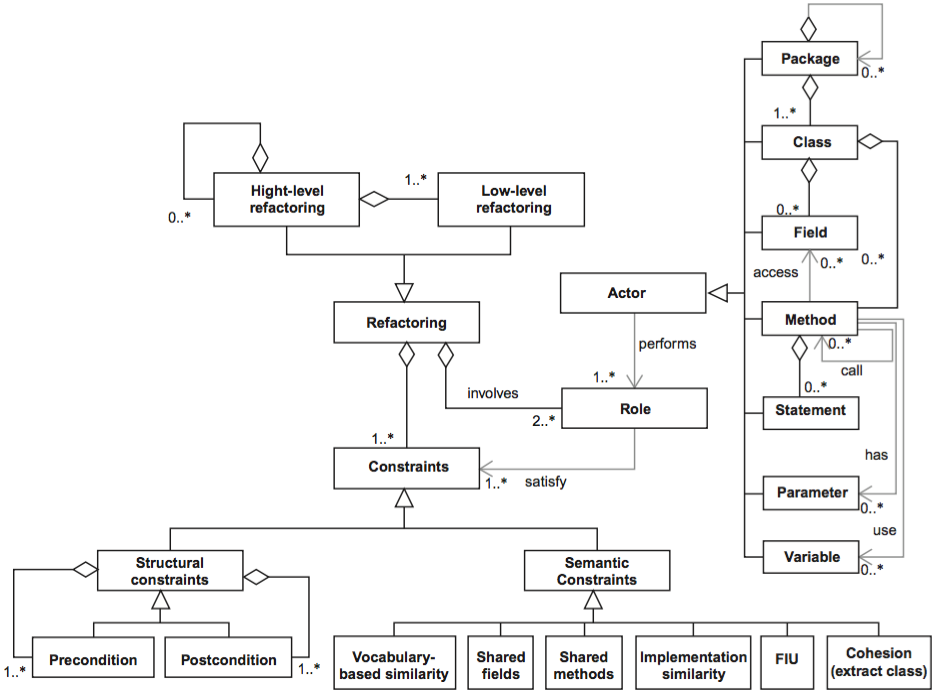
\includegraphics[scale=0.45]{images/metamodelo_refatoracao_related}
	\fadaptada{ouni2014_multiobjective}
\end{figure}

Para aplicar uma refatoração é necessário especificar qual elemento estrutural é envolvido/impactado pela refatoração. De acordo com os autores, o elemento estrutral é especificado pela supermetaclasse \texttt{Actor} e suas submetaclasses: \texttt{Package}, \texttt{Class}, \texttt{Field}, \texttt{Method}, etc. No SRM o engenheiro de modernização também deve especificar quais são os elementos estruturais que são envolvidos na operação da refatoração. Porém, tais elementos estruturais são representados por metaclasses do metamodelo KDM - fazendo com que as refatorações especificadas no SRM sejam independente de linguagem e plataforma. 

Como observado na Figura~\ref{fig:refactoring_metamodel_related} o metamodelo proposto por~\citeonline{ouni2014_multiobjective} possui dois tipos de restrições: (\textit{i}) \texttt{Structural Constraints} e (\textit{ii}) \texttt{Semantic Constraints}. O SRM contém apenas três metaclasses para representar as restrições da refatoração, ou seja, a supermetaclasse \texttt{Constraint} e as submetaclasses \texttt{PreCondition} e \texttt{PostCondition}. Porém, o SRM permite que o engenheiro de modernização especifica restrições em OCL ou XQuery. Além disso, a principal diferença entre o SRM e o metamodelo proposto por~\citeonline{ouni2014_multiobjective} é que o SRM tem como objetivo não especificar e documentar refatorações. O SRM permite compartilhar refatorações e prover a interoperabilidade entre diversas ferramentas, assim, qualquer ferramenta que utilize o metamodelo KDM, poderá utilizar as refatorações definidas pelo SRM.

\begin{figure}[h]
	\centering
	% Requires \usepackage{graphicx}
	\caption{\textit{Structured Metrics Metamodel} - SMM.}
	\label{fig:SMM_metamodel_related}
	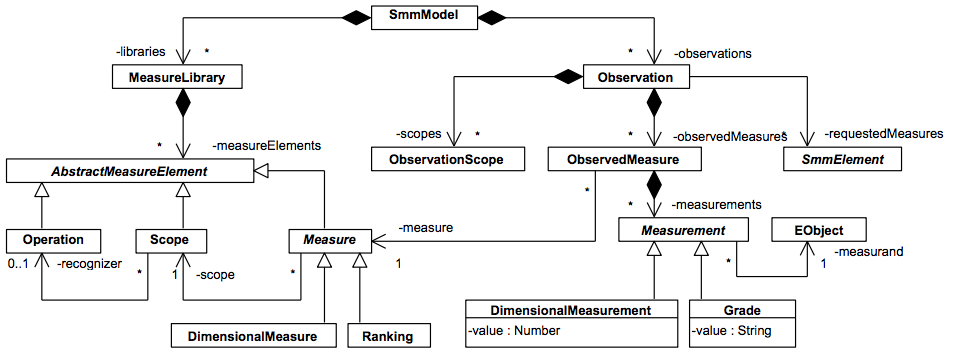
\includegraphics[scale=0.45]{images/SMM_metamodelo_related}
	\fadaptada{ADM:SMM}
\end{figure}

Não foi encontrado outro metamodelo similar ao SRM. No entanto, na literatura é possível identificar o metamodelo SMM, o qual é uma padronização da ADM e é utilizado para especificar métricas de software~\cite{ADM:SMM}. A ideia é similar ao metamodelo SRM por isso o metamodelo SMM foi considerado um trabalho relacionado. O SMM é um metamodelo que proporciona um formato padrão tanto para definir métricas quanto para representar os resultadas das medições. O SMM é apresentado na Figura~\ref{fig:SMM_metamodel_related}. As principais metaclasses do SMM são: \texttt{Measures} (métricas) e \texttt{Measurements} (medições). A metaclasse \texttt{Measures} descreve uma maneira para calcular propriedades de um sistema. A metaclasse \texttt{Measurements} representa medições, mais especificamente resultados da aplicação de uma métrica em um modelo alvo a ser medido.

Existem algumas vantagens no uso do SMM. Além de ser um metamodelo para métricas e medições proposto pela ADM, ele se faz vantajoso pelo fato de ser um padrão, logo, métricas definidas em conformidade com o metamodelo SMM podem ser testadas, reusadas e compartilhadas da mesma forma que o SRM pode prover o compartilhamento de refatorações. Além disso, o uso de um padrão facilita o desenvolvimento de ferramentas compatíveis capazes de automatizar o processo de medição~\cite{ADM:SMM}.

Outro metamodelo relacionado ao SRM é o metamodelo \sigla{SPMS}{\textit{Structured Patterns Metamodel Standard}}~\cite{ADM:SPMS}. Esse metamodelo é utilizado para representar padrões de software, tais como: \textit{anti-patterns}, \textit{design patterns}, \textit{architectural patterns}, \textit{build patterns} e etc.SPMS fornece um conjunto de metaclasses para instanciar diversos padrões de software. Uma visão geral do metamodelo SPMS é apresentado na Figura~\ref{fig:SPMS_metamodel_related}. 

\begin{figure}[h]
	\centering
	% Requires \usepackage{graphicx}
	\caption{\textit{Structured Patterns Metamodel Standard} - SPMS.}
	\label{fig:SPMS_metamodel_related}
	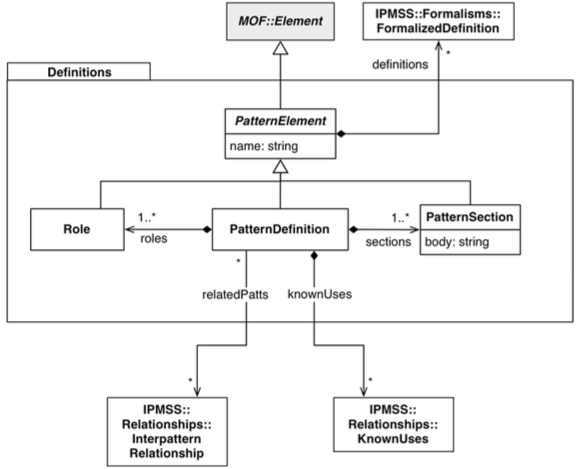
\includegraphics[scale=0.57]{images/SPMS_related}
	\fadaptada{ADM:SPMS}
\end{figure}

A metaclasse \texttt{PatternElement} possui meta-atributos para representar o padrão que se almeja instanciar. \texttt{Role} é uma metaclasse para representar elementos conceituais que um determinado padrão necessita. A metaclasse \texttt{PatternDefinition} é uma submetaclasse de \texttt{PatternElement} e possui duas composições: (\textit{i}) \texttt{sections} do tipo \texttt{PaternsSection} e (\textit{ii}) knownUses do tipo \texttt{KnownUses}. Além disso, a metaclasse \texttt{PatternDefinition} tem uma dependência denominada \texttt{relatedPatts} do tipo \texttt{InterPatternRelationship} que representa os padrões internos que um padrão pode possuir.


\section{Considerações Finais}
\label{sec:consideracoes_finais_SRM}

Refatorações são de suma importância durante a manutenção, produção e análise de software. Inúmeras comunidades têm surgido na literatura para criar e definir vários tipos de refatorações, incluindo refatorações de baixa granularidade~\cite{Fowler1999, Demeyer1, Demeyer2}, refatorações arquiteturais, refatorações para o paradigma orientado a aspecto, etc. 

Neste contexto, há uma grande necessidade da definição de um padrão para auxiliar e promover o compartilhamento dessas refatorações, tanto dentro como entre estas comunidades. Como uma iniciativa para suprir tal limitação neste capítulo foi apresentado o metamodelo SRM para auxiliar o engenheiro a promover o reuso de refatorações. O SRM está inserido no contexto da ADM para preencher a definição de um metamodelo de refatorações. Assim, com a utilização desse metamodelo, metadados sobre refatorações podem ser reutilizadas de forma independente de linguagem e plataforma.

O SRM contém 13 metaclasses e quatro enumerações e foi implementado utilizando o EMF. Para a representação dos elementos estruturais que são utilizados durante uma refatoração o metamodelo KDM foi utilizada. O mecanismo/operação da refatoração são representados utilizando a linguagem de transformação ATL e/ou QVT. As restrições que devem ser satisfeitas antes e após a condução da refatoração são representadas por meio de OCL e/ou XQuery. A fim de utilizar plenamente as vantagens dos metamodelo SRM, os engenheiros de modernização precisam ter um bom conhecimento de linguagem de programação avançada. Na verdade o engenheiro deve estar familiarizado como as semânticas das refatorações (por exemplo, qual(is) é (são) o(s) pré-requisito(s) para a execução de uma refatoração) e como/onde utilizar e programar tais refatorações. Além disso, a instanciação de uma refatoração utilizando o SRM é bastante verbosa, complexa e propensa a erros, uma vez que exige o conhecimento avançado de refatoração e habilidades de programação em relação a API Ecore, uma vez que o SRM foi desenvolvido utilizando o EMF. Neste contexto, foi criado e apresentado neste capítulo um conjunto de gramáticas que quando compostas derivam uma DSL, a qual é utilizada para facilitar a utilização e instanciação do metamodelo SRM. Uma visão geral da DSL, bem como utilizá-la também foi apresentada neste capítulo. O editor resultante pode ser observado no Capítulo~\ref{chapter:ferramenta_kdm_re}. % por meio da ferramenta denominada KDM-RE que possui um módulo que defini uma DSL para facilitar a instanciação e reutilização de do metamodelo SRM. No Capítulo~\ref{chapter:avaliacao} é discuto um experimento que foi realizado para avaliar as refatorações e a ferramenta KDM-RE.

%No próximo capítulo é apresentado uma abordagem denominada KDM-SInc para realizar a propagação de mudança e preservação de comportamento após a aplicação de refatorações em instâncias do metamodelo KDM. 


